\documentclass[conference]{IEEEtran}

% \IEEEoverridecommandlockouts
% The preceding line is only needed to identify funding in the first footnote. If that is unneeded, please comment it out.

% %%%%%%%%%%%%%%%%%%%%%%%%%%%%%%%%%%%%%%%%%%%%%%%%%%%%%%%%%%%%%%%%%%%%%%%%%%%%%
% Packages
% %%%%%%%%%%%%%%%%%%%%%%%%%%%%%%%%%%%%%%%%%%%%%%%%%%%%%%%%%%%%%%%%%%%%%%%%%%%%%

\usepackage{cite}
\usepackage{amsmath,amssymb,amsfonts}
\usepackage{algorithmic}
\usepackage{graphicx}
\usepackage{textcomp}
\usepackage{xcolor}
\usepackage{listings}
\lstset{
    language=C++,                                     % choose the language of the code
    basicstyle=\scriptsize\ttfamily,basewidth=0.75em, % the size of the fonts that are used for the code
    numbers=left,                   % where to put the line-numbers
    numberstyle=\scriptsize,        % the size of the fonts that are used for the line-numbers
    stepnumber=1,                   % the step between two line-numbers. If it is 1 each line will be numbered
    numbersep=5pt,                  % how far the line-numbers are from the code
    backgroundcolor=\color{white},  % choose the background color. You must add \usepackage{color}
    showspaces=false,               % show spaces adding particular underscores
    showstringspaces=false,         % underline spaces within strings
    showtabs=false,                 % show tabs within strings adding particular underscores
    frame=single,                   % adds a frame around the code
    tabsize=2,                      % sets default tabsize to 3 spaces
    captionpos=b,                   % sets the caption-position to bottom
    breaklines=true,                % sets automatic line breaking
    breakatwhitespace=false,        % sets if automatic breaks should only happen at whitespace
    linewidth=\columnwidth,
    boxpos=b,
    xleftmargin=2em,
    framexleftmargin=1.5em,
    %escapeinside={\%
    %}
    %{
    %)}          % if you want to add a comment within your code
}
\def\BibTeX{{\rm B\kern-.05em{\sc i\kern-.025em b}\kern-.08em
    T\kern-.1667em\lower.7ex\hbox{E}\kern-.125emX}}

% %%%%%%%%%%%%%%%%%%%%%%%%%%%%%%%%%%%%%%%%%%%%%%%%%%%%%%%%%%%%%%%%%%%%%%%%%%%%%
% Begin Document
% %%%%%%%%%%%%%%%%%%%%%%%%%%%%%%%%%%%%%%%%%%%%%%%%%%%%%%%%%%%%%%%%%%%%%%%%%%%%%

\begin{document}

% %%%%%%%%%%%%%%%%%%%%%%%%%%%%%%%%%%%%%%%%%%%%%%%%%%%%%%%%%%%%%%%%%%%%%%%%%%%%%
% Title
% %%%%%%%%%%%%%%%%%%%%%%%%%%%%%%%%%%%%%%%%%%%%%%%%%%%%%%%%%%%%%%%%%%%%%%%%%%%%%

\title{Spectrum: Classifying, Replicating and Mitigating Spectre Attacks on a Speculating RISC-V Microarchitecture}

% %%%%%%%%%%%%%%%%%%%%%%%%%%%%%%%%%%%%%%%%%%%%%%%%%%%%%%%%%%%%%%%%%%%%%%%%%%%%%
% Authors
% %%%%%%%%%%%%%%%%%%%%%%%%%%%%%%%%%%%%%%%%%%%%%%%%%%%%%%%%%%%%%%%%%%%%%%%%%%%%%

\author{\IEEEauthorblockN{Gonzalez, Abraham}
\IEEEauthorblockA{\textit{CS 262A}\\ \textit{CS 294-156}} \\
\and
\IEEEauthorblockN{Korpan, Ben}
\IEEEauthorblockA{\textit{CS 262A}\\ \textit{CS 294-156}} \\
\and
\IEEEauthorblockN{Younis, Ed}
\IEEEauthorblockA{\textit{CS 262A}\\ \textit{CS 261}} \\
\and
\IEEEauthorblockN{Zhao, Jerry}
\IEEEauthorblockA{\textit{CS 294-156}} \\
}

\maketitle

\begin{abstract}
    With the discovery of speculative execution exploitative attacks the computer
    architecture community is rethinking the architecture boundry and how the
    attacks can be mitigated. This project aims to tackle this new set of problems
    by providing three different outcomes; a comphrehensive taxomony for attacks
    and defenses, replication of speculative attacks on an open-source processor,
    and a mitigation developed for some of these attacks on an open-source
    processor.
    
    We have categorizaed the variety of attacks based on if the attacks are 
    architecturally legal and the defenses based on their types. Additionally, 
    for the taxonomy we have mapped mitigations to the proper attacks that they 
    potentially cover. Using the Berkeley Out-Of-Order Machine, we have 
    reimplemented Spectre Variants 1 and 2 that target the L1 Data Cache. We 
    achieve a leakage rate of around 114 bytes per sec with a 100MHz processor 
    frequency. For mitigating these speculative load type of attacks, we 
    implemented a speculative buffer that resides within the MSHRs. Based on
    preliminary results, it achieves a 2151 score on the Dhrystone benchmark
    resulting in a 1\% performance decrease compared to the baseline. Additionally,
    synthesizing around a 45nm process shows a 3\% area increase and 3\% lower clock
    impact.
\end{abstract}

\section{Introduction}

Ever since the disclosure of Spectre and Meltdown at the beginning of 2018, there has
been a large number of attacks targeting speculative microarchitectural state in
out-of-order processors \cite{b1,b2}. Each of these attacks is able to exploit the shared
state of the processor between a victim process/thread and a malicious process/thread.
While classifications have been developed for cache-based and for timing-based 
side-channel attacks \cite{b5,b6,b7,b9,b10}, a general taxonomy for these attacks has not been adopted.
A well-devised taxonomy would inform not only the 
categorization of new attacks but also the development of hardware mitigations for 
these attacks. A complete categorization system would help hardware researchers 
identify general mitigations for broad categories of vulnerabilities, instead of 
targeted fixes for specific attacks. Additionally, the Berkeley Out-of-Order Machine (BOOM) open-source RISC-V
microarchitecture has not been exposed to these types of attacks yet \cite{b11}. BOOM
is a generic implementation of a speculative 
out-of-order microarchitecture that employs many of the same features as the 
proprietary systems targeted by published attacks. Generic, open-source 
implementations of attacks and their mitigation strategies would provide a common 
foundation for the development of defenses for speculative execution attacks.
By attacking an open-source machine with Spectre, researchers can not only gain more 
insight into the malicious attack but also attempt to mitigate the attack on a shared,
open platform. Moreover, this project is hoped to unify and guide the attack 
mitigation process. With an attack taxonomy and an open-source microarchitecture, a 
newly proposed mitigation technique can easily target a class of attacks as informed 
by the taxonomy.

The remainder of this paper is structured as follows: In Section 2, we discuss
related works that indicate relevant work that introduces attacks, defenses, and classifications.
In Section 3 we discuss our taxonomy and how we think about the attacks and defenses. In
Section 4 we present the subset of attacks that were replicated for this paper. In Section 5
we discuss the implementation of the SpecBuf. In Section 6 we discuss the evaluation of the
replications and the SpecBuf. In Section 7 we discuss future work that can be done with each
component and conclude in Section 8.

\section{Related Works} \label{Related Works}

\subsection{Speculative Style Attacks}

\subsubsection{Spectre}

This work first described speculative style attacks on out-of-order cores that 
allow a malicious user to read secret data from a victim \cite{b1}. When an out-of-order 
processor reaches a control flow instruction, it predicts the direction of program flow
using the Branch Target Buffer and Branch Predictor.
If the control flow is mispredicted, then the code that was
executed will not be committed into the architectural state. However, data leakages can 
occur due to the speculated instruction changing the microarchitectural state.
This work introduced two main variants that leak secret data through
a cache side channel attack. The first variant named Bounds Check Bypass
trains the Branch Predictor to ignore a bounds check and retrieve secret data. The
second variant uses the Branch Target Buffer to determine which target to execute
called a gadget. Both attacks exploit speculative execution and thus
affect all types of out-of-order speculative microarchitectures.
Therefore, significant changes to the microarchitecture and software stack will have
to occur to mitigate these attacks.
Our work serves as an extension of this result by categorizing, replicating, and mitigating
speculative cache side channel attacks on an open source out-of-order microarchitecture.

\subsubsection{Meltdown}

This work describes another speculative attack where an attacker 
can bypass privilege levels and read all the data from kernel memory \cite{b2}.
This attack uses speculated code run after a memory access
protection exception to leak kernel memory to the attacker. When a kernel memory 
location is accessed in a lower privilege level, then the privilege check occurs
in parallel with retrieving the data. Thus, when this data is retrieved, the following
instructions can be speculatively executed, leaking the information through a side
channel. This type of attack
is more dangerous than Spectre in that it leaks kernel memory (and physical memory if
it is mapped in the kernel), however, it is easier to mitigate through mechanisms such
as KAISER \cite{b21} which unmaps the physical memory from the kernel preventing the attack.
Our work for this paper addresses the leakage mechanism of this particular attack but 
does not solve the source of the attack since it is specific to x86 architectures.

\subsection{Speculation Defenses}

\subsubsection{InvisiSpec}

InvisiSpec is a theoretical implementation of a speculative buffer on a multi-core
processor \cite{b46}. This buffer is designed to extend the Load Queue (LQ) and hold all unsafe speculative loads.
Since InvisiSpec's buffer is invisible to the memory hierarchy, the buffer is
invisible to the cache coherence protocol. This implies that the hardware must track cache
coherence requests that effect speculated loads and apply them correctly and safely. This is
done with an exposure scheme that enforces memory consistency and cache coherence protocols.
InvisiSpec achieves a 72\% slowdown during software simulation. Our implementation differs by only
considering a single-core processor which allows us to ignore cache coherence. Additionally, we extended the Miss
Status Holding Registers (MSHRs) instead of the LQ to achieve practical and synthesizable results
rather than InvisiSpec's buffer that assumes infinite area and size.

\subsubsection{SafeSpec}

SafeSpec is another theoretical implementation of a speculative buffer on an x86 processor \cite{b29}.
Unlike InvisiSpec and our work, SafeSpec considers adding speculative buffers to the Translation Lookaside Buffer and 
L1 caches which results in significant control flow changes.
Simulated CPU results show an 26.4\% power and 17\% area overhead in the worst case. One
important contribution of SafeSpec is the paper's discussion on side channels using the speculative
buffer. With the buffer, the side channels are a few orders of magnitude more difficult and inefficient to perform.
We differ from this work by creating a working implementation of a speculative buffer that protects the data cache.

\subsection{Other Classifications}

\subsubsection{A Systematic Evaluation of Transient Execution Attacks and Defenses}

This work proposes a systematic classification for speculative attacks \cite{b48}. 
In addition to categorizing the attacks, the authors also described other undiscovered speculative attack variants.
Additionally, this paper does a in-depth analysis of Spectre-type mitigations, but has a very short evaluation of Meltdown defenses.
Our taxonomy differs from this work by mainly focusing on a vendor agnostic solutions to speculative side channel attacks.

\section{Speculative Attack Replication} \label{Speculative Attack Replication}

To our knowledge, speculative attacks have not yet been implemented on BOOM. Thus,
one of the goals of this project was to demonstrate simple proof of concept implementations for a
subset of speculative style attacks. Originally, the goal was to implement both 
Spectre-v1, otherwise know as the Bounds Check Bypass attack, and the Return Stack Buffer attack \cite{b3}.
However, due to the instability of BOOM's high-performance branch predictors, the team instead implemented
proof of concepts for Bounds Check Bypass attack and Spectre-v2, otherwise known as the
Branch Target Injection attack. Over 520 lines of code were written for both implemented attacks as well as 
code for the untested Return Stack Buffer attack. The source code for these replicated attacks is available at
\url{https://github.com/riscv-boom/boom-attacks}.

\subsection{Implementation Details}

This project utilizes the Berkeley Out-of-Order Machine (BOOM), a synthesizable and 
parameterizable open source RV64G RISC-V core written in the Chisel hardware construction language \cite{b49}. 
The microarchitecture is open source, providing insight into the front-end and memory system
used. The ability to introspect on the inner mechanics of the core enabled us to quickly replicate 
the attacks and maximize their performance. We describe some of the issues encountered in this process:

\subsubsection{Flushing a cache line}

One feature of the popular x86 and ARM ISAs is the availability of cache manipulation instructions
(for example x86 has {\tt clflush} to flush a cache line from every level of the cache hierarchy).
However, RISC-V does not have a corresponding {\tt clflush} equivalent.
This type of instruction is extremely important for cache side channel attacks since it allows for
the attacker to precisely control the contents of the cache.
Therefore, a workaround was made to implement an equivalent
L1 cache line flush function. This function takes in an address and size in bytes, and flushes
all sets starting from that address until the size. This is done by having an extra array which 
is a multiple of the L1 cache size, that when indexed into, evicts a cache line within the set that the input
address refers to.

While {\tt clflush} is able to selectively remove a cache line from the cache without 
affecting the rest of the cache state, the function created is only able to evict the entire set.
This enforces that the cache line referenced is evicted at the cost of evicting other lines, causing a performance
decrease. Evicting the entire set is done by accessing the extra array addresses corresponding to the set 
{\tt N * L1\_WAY} times, where {\tt N} is large enough to account for the random cache replacement policy. The larger
the {\tt N} value, the higher probability that the particular cache line is evicted from the set. For our purposes, this value
was chosen to be {\tt N = 4} in order to have a 99\% probability of evicting the referenced cache line.

\subsubsection{BOOM Branch Predictor Unit}

% TODO: double check that the ghr is hashed and folded

The BOOM Branch Predictor Unit (BPU), is split into a single-cycle "next-line predictor" (NLP) and a
slower but more complicated "backing predictor" (BP). The NLP contains the Branch Target Buffer (BTB) 
where more recent branches are cached alongside their target, a tag of the PC, and more metadata. Additionally,
the NLP contains the Return Stack Buffer (RSB) which holds the return pointer for a {\tt ret} instruction. The BP
consists of a large predictor such as a TAGE or GShare predictor which makes a more accurate prediction based on
a larger view of the branch history \cite{b47}. For simplicity, the team used a GShare predictor, since it is 
easier to train and was fully functioning at the start of the project. The GShare predictor had a global history of 23 bits and history table containing 4096 
counters. Since the global history was longer than the size of the table, the global history was hashed with the 
instruction PC and folded to index into the history table. Additionally, when trying to
implement the RSB attack, it was discovered that the RSB was disabled causing all {\tt ret} instructions
to speculate to the next PC instead of the return target PC. Re-enabling the RSB led to multiple other BPU bugs,
so we decided to keep the RSB disabled and instead implement the Branch Target Injection attack.

\subsubsection{BOOM Memory System}

% TODO: does this make sense to people

BOOM's memory system utilizes the RocketChip L1 Data Cache and connects to the rest of the RocketChip
uncore \cite{b54}. However, in the configuration of BOOM used, there is a L1 cache and outer memory set to a L2 cache
latency. This memory hierarchy still functions properly, however it was noticed that the speculation window
was not large enough due to the memory model mandating that the latency to any memory request would be no greater than latency to L2.
While a real attack would use L2 or L3 cache misses to expand the speculation window, we instead approximated this with a {\tt fdiv} dependency chain.

\subsection{Bounds Check Bypass Attack} \label{Bounds Check Bypass Attack}

In this attack, the attacker resides in the same address space as the victim and uses
conditional branches to read victim data. The attacker would first train a conditional branch
within the victim code to predict the branch to be taken in a certain direction. Then,
during the attack round, the attacker
gives a value to the victim that fails the bounds check in the victim but during
speculation is used to retrieve the secret value. This particular attack variant
uses a cache side channel attack to leak the information by having a passed in value retrieve
a secret value which is then used to index the "attacker array". After the attack is run, this 
"attacker array" can be scanned and timed to determine the secret value based on the timings
of cache hits. The psuedocode for this type of attack in Code \ref{code:spectre-v1-pseudo}
demonstrates the attack concept using a C-like syntax.

\begin{lstlisting}[style=column-code, label={code:spectre-v1-pseudo}, caption=Psuedocode of Bounds Check Bypass Attack]
char* secret[] = "SECRET_VALUE"
char  attackArray[256 * CACHE_BLOCK_SZ]

void victim(idx){
  if (idx < secret.size())
    attackArray[secret[idx] * CACHE_BLOCK_SZ]
}

int main(void){
  // Train BPU and Attack secret value
  while (TRAINING_ROUNDS)
    victim(idx)

  victim(outOfBoundsIdx)

  // Probe array to check for hit
  for (i -> 0 until 256){
    t0 = time()
    attackArray[i * CACHE_BLOCK_SZ]
    t1 = time()
  }
}
\end{lstlisting}

% TODO: double check the bpu hashing

The BOOM implementation of this attack echos the Spectre-v1 proof of concept and the psuedocode closely.
It consists of three different parts. First, a tally buffer is cleared before reading a secret byte.
This tally buffer is used to keep track of the amount of hits a secret value gets during the measurement
phase. Next the array to be probed is evicted from the cache (the "attacker array" mentioned above), and
the attacker trains the BPU to enter the bounds protected area within the victim function. Note that in
this section, there is an extra loop that puts the branch history in a consistent state since the branch
history is hashed on update. Finally, the attacker code reads out the probing array through using the
{\tt rdcycle} instruction and checks if the result is under a hand tuned cache threshold. Full code for 
this attack is at Code \ref{code:boom-spectre-v1}.

\subsection{Branch Target Injection Attack}

This attack exploits the outcome
of {\tt jalr} instructions which use the BTB to predict the destination. In this attack,
the attacker trains a BTB entry for a {\tt jalr} instruction to point to 
the victim code. Then during the attack run, when the {\tt jalr} is supposed to go to another function,
the BTB redirects the PC to the victim code where it speculatively leaks the secret value. Similar to the
Bounds Check Bypass attack, this attack leaks information through the
cache side channel mentioned in Section \ref{Bounds Check Bypass Attack}. The psuedocode in 
Code \ref{code:spectre-v2-pseudo} demonstrates the basic principle of the attack using a C-like syntax.

\begin{lstlisting}[style=column-code, label={code:spectre-v2-pseudo}, caption=Psuedocode of Bounds Check Bypass Attack]
char* secret[] = "SECRET_VALUE"
char  attackArray[256 * CACHE_BLOCK_SZ]

void otherFunction(void){
  // Other functionality    
}

void victim(idx){ attackArray[secret[idx] * CACHE_BLOCK_SZ] }

int main(void){
  
  // Training
  while (TRAINING_ROUNDS){
    jump(victim)
  }

  // Attack. Read secret value
  argument = attackIdx
  jump(otherFunction)

  // Probe array to check for hit
  for (i -> 0 until 256){
    t0 = time()
    attackArray[i * CACHE_BLOCK_SZ]
    t1 = time()
  }
}
\end{lstlisting}

The BOOM implementation of this attack is very similar to the implementation given for
the Bounds Check Bypass attack listed in Section \ref{Bounds Check Bypass Attack}. One of the main differences
for this attack is that the attacker has to change both the address of the function being called through
{\tt jalr} and the passed in value to the victim function throughout the training and the attack run.
Another difference between the two attacks is that the {\tt fdiv} manipulation is instead done on the target address
in the main function instead of using {\tt fdiv} on the passed in index in the victim code.

\input{defense}
\section{Proposed Taxonomy}
\begin{itemize}
	\item Looked at it from perspective of architecture
	\item Attacks
		\begin{itemize}
			\item First Split on Architecture Legal, reason: bug needing bugfix or not
			\item If illegal, split on fault type, reason: obvious
			\item If pagefault, further split on page permission bit, reason: obvious
			\item If legal, split on hardware buffer affected, reason: the module that needs to be rethought
		\end{itemize}

	\item Defenses
		\begin{itemize}
			\item defenses were catergorized based on implementation where, how much, when, etc
			\item First split on where is defense implemented, reason: determine what you can implement new hardware vs new compiler
			\item Firmware - microcode changes, pick and choose if it applies
			\item Software further split on OS or App, reason: Do you have control over OS, can you control OS, do you trust OS, answer no to any look at App level fixes
			\item Hardware futher split on change to existing hardware or completely new concept, reason: implementation cost
		\end{itemize}

\end{itemize}

\begin{center}
\begin{figure}[!p]
    \makebox[\textwidth]{\includegraphics[width=1.1\paperwidth,angle=270]{categorization}}
    %\captionsetup{justification=centering}
    \caption{Full taxonomy of different attacks and defenses and what they cover}
    \label{fig:categorization}
\end{figure}
\afterpage{\clearpage}
\end{center}

\section{SpecBuf}
The side-channel which forms the basis of multiple Spectre variants is the modification of data cache state during speculative execution.
To improve performance, modern out-of-order cores will speculatively fetch data into the core on a load miss.
However, in the event that the load miss is misspeculated, the refill data is still written into the cache, potentially evicting other resident cache lines.
By carefully measuring the execution times of repeated loads, attacker code can inspect the state of the cache and infer the destination addresses of misspeculated loads by the victim code.

To address this issue, the tag and data arrays must be considered as part of the ``architectural state'' of the machine, since their contents will affect the ``architectural'' results of timing measurements performed by attacker code.
Similar to how architectural register state is managed in the execution pipelines of out-of-order machines, a secure core must only allow correctly speculated, committing instructions to modify the cache state.
A proposed approach is to hold speculated load data in an ``L0 Speculation buffer'' that can be flushed when misspeculation is realized.
This prevents misspeculated loads from affecting the state of the cache, while still allowing correctly speculated loads to broadcast their data into the rest of the machine as soon as possible, maintaining performance. If well implemented, such a buffer could slightly improve performance by deferring the eviction of prior contents, slightly reducing the miss latency, and could even be combined with a store coalescing buffer - another useful ``L0 buffer'' structure.

\subsection{Miss Status Holding Registers}
\begin{figure}
  \begin{center}\includegraphics[scale=0.17]{dcache.png}\end{center}
  \caption{Design of modified L1 data cache}
\end{figure}

We implement such a speculation buffer as part of the Miss Status Holding Registers (MSHRs) in BOOM's L1 data cache. The MSHRs hold the status of inflight memory requests made by the L1 cache to the L2 memory bus.
In the original data cache, L2 cache refills would write the refill data into the tag and data arrays before waking up the corresponding MSHRs to return the load data to the core.
To implement a speculation buffer, we modified cache refills to instead write the refill data into per-MSHR cacheline buffers.

On misspeculation, the misspeculated MSHR entry is flushed along with any load data that has been returned. Only after the load which allocated the MSHR entry is known to be committed is the new cacheline written into the tag and data arrays. This effectively prevents misspeculated loads from altering the state of the cache.

Since speculating past loads is necessary for performance, we allow bypassing request data out of the speculation buffer, before the data is committed into the tag and data arrays. The consequence of this bypassing is that the service time for a cache miss is unchanged from the original behavior.

Another subtlety of the MSHRs is the per-MSHR replay queues, which hold subsequent requests to the same cache-line. These queues are necessary for handling consecutive load misses to the same cacheline without occupying more valuable MSHR entries. Our speculation buffer will eagerly empty the replay queues until a store miss is seen in the queue. Since stores issued to the memory system are always non-speculative, the cacheline can be immediately committed.

\subsection{MSHR Optimization}


\subsection{Point of No Return}
In the naive implementation of the speculation buffer, entries in the buffer are only deallocated when the instruction is reached by the head of the reorder buffer (ROB). However, this can result in heavy MSHR utilization, since there may be many instructions between a waiting load and the commit head waiting to execute and write back. However, we observe that many of those instructions, while still inflight, can be marked as guaranteed to commit.

This leads to the concept of a ``point-of-no-return'' (PnR) in the ROB, in addition to the commit head. While the commit head tracks the next instruction which will commit the architectural state, the PnR tracks instructions which are guaranteed to eventually commit, even if they have not yet completed execution. In other words, the PnR points at the oldest instruction which may cause misspeculated execution; an unsafe instruction, such as a branch which has not yet executed. If an instruction is marked as safe, the PnR will pass it whether or not it has completed executing. We observe that refills in the spec-buffer can be committed to the cache as soon as the PnR passes the instruction which triggered them. This reduces pressure on MSHR resources and prevents backpressure on incoming cache requests.

To reduce the performance impacts of our speculation buffer, we implemented a PnR in the ROB. Two versions were implemented. The first simple-PnR is a less expensive pointer that will only mark at most one ROB row per cycle as ``guaranteed to commit''. We also implemented a more complex PnR head that can mark an arbitrary number of rows per cycle, essentially ``jumping over'' groups of safe instructions to the oldest instruction unsafe.

\section{Evaluations} \label{Evaluations}

\subsection{Base Core Parameters}

The two different attacks were replicated on the BOOM core with the parameters given
in \ref{tab:boom-core-params}. All attacks were measured using FireSim, an open-source
cycle-accurate, FPGA-accelerated scale-out computer system simulation platform \cite{b12}.

\begin{table}
\centering \caption{BOOM Core Parameters} \label{tab:boom-core-params}
\begin{tabular}{@{} *2l @{}} \toprule
    Parameter                    & Value \\ \midrule
    Fetch Width                  & 2 \\
    Decode Width                 & 2 \\
    Issue Width                  & 4 \\
    PRF Size                     & 100 \\
    ROB Size                     & 100 \\ \midrule
    L1 Sets                      & 64 \\
    L1 Ways                      & 8 \\
    L1 Linesize                  & 64 bytes \\ \midrule
    BTB Sets                     & 512 \\
    BTB Banks                    & 2 \\
    BTB Ways                     & 4 \\ \midrule
    GShare History Bits          & 23 \\
    GShare Counter Table Entries & 4096 \\ \bottomrule
\end{tabular}
\end{table}

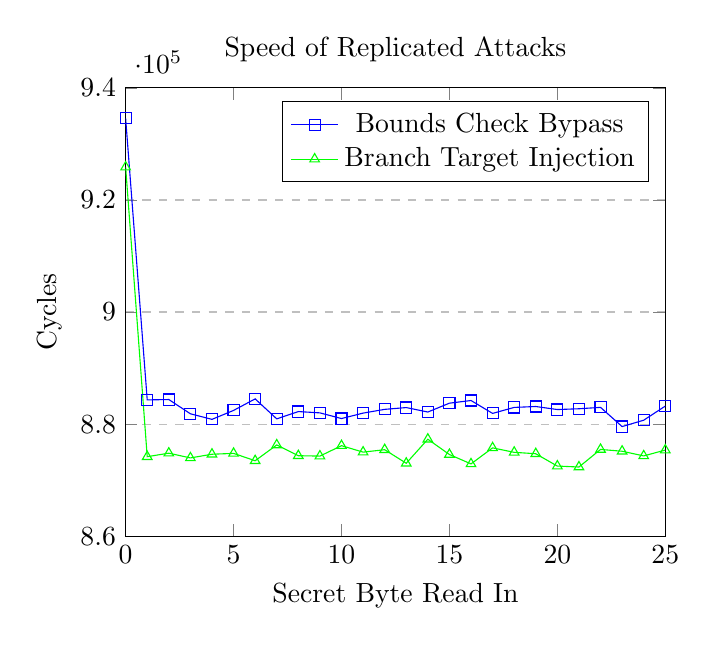
\begin{tikzpicture}
\begin{axis}[
    title={Speed of Replicated Attacks},
    ylabel={Cycles},
    xlabel={Secret Byte Read In},
    xmin=0, xmax=25,
    ymin=860000, ymax=940000,
    legend pos=north east,
    ymajorgrids=true,
    grid style=dashed
]

\addplot[
    color=blue,
    mark=square,
]
coordinates {
    (0 ,934580)
    (1 ,884322)
    (2 ,884387)
    (3 ,881845)
    (4 ,880847)
    (5 ,882446)
    (6 ,884498)
    (7 ,880939)
    (8 ,882241)
    (9 ,882006)
    (10,880994)
    (11,881965)
    (12,882634)
    (13,882954)
    (14,882156)
    (15,883738)
    (16,884212)
    (17,881912)
    (18,882980)
    (19,883142)
    (20,882600)
    (21,882739)
    (22,882989)
    (23,879563)
    (24,880698)
    (25,883218)
};
        
\addplot[
    color=green,
    mark=triangle,
]
coordinates {
    (0 ,925862)
    (1 ,874188)
    (2 ,874815)
    (3 ,873968)
    (4 ,874626)
    (5 ,874778)
    (6 ,873466)
    (7 ,876281)
    (8 ,874361)
    (9 ,874297)
    (10,876153)
    (11,875000)
    (12,875435)
    (13,873015)
    (14,877303)
    (15,874572)
    (16,872902)
    (17,875761)
    (18,874966)
    (19,874715)
    (20,872514)
    (21,872346)
    (22,875481)
    (23,875161)
    (24,874325)
    (25,875371)
};
\legend{Bounds Check Bypass,Branch Target Injection}

\end{axis}
\end{tikzpicture}


\begin{lstlisting}[style=column-code, caption=Printout of Bounds Check Bypass Attack]
want(!) =?= 1.(!) 2.(^A)
want(") =?= 1.(") 2.(^A)
want(#) =?= 1.(#) 2.( C)
want(T) =?= 1.(T) 2.(^A)
want(h) =?= 1.(h) 2.(i)
want(i) =?= 1.(i) 2.(>)
want(s) =?= 1.(s) 2.(^D)
want(I) =?= 1.(I) 2.(^D)
want(s) =?= 1.(s) 2.( ^L)
want(T) =?= 1.(T) 2.( )
want(h) =?= 1.(h) 2.(^F)
want(e) =?= 1.(e) 2.()
want(B) =?= 1.(B) 2.(<9f>)
want(a) =?= 1.(a) 2.(^B)
want(b) =?= 1.(b) 2.(^A)
want(y) =?= 1.(y) 2.()
want(B) =?= 1.(B) 2.( )
want(o) =?= 1.(o) 2.(^H)
want(o) =?= 1.(o) 2.(4)
want(m) =?= 1.(m) 2.(k)
want(e) =?= 1.(e) 2.(^C)
want(r) =?= 1.(r) 2.(^A)
want(T) =?= 1.(T) 2.(^C)
want(e) =?= 1.(e) 2.(^O)
want(s) =?= 1.(s) 2.(^D)
want(t) =?= 1.(t) 2.(^A)
\end{lstlisting}
\label{code:spec-attack-printout}

\subsection{Replicating Speculative Attacks Results}

Overall, the attacks chosen were replicated successfully on the BOOM microarchitecture. A printout
demonstrating leakage of secret information with the Bounds Check Bypass attack
is shown in \ref{code:spec-attack-printout}. Initial results of the replications
are promising with around 3.6KB/s for both attacks. \ref{tab:spec-attack-results}
shows the results of the two attacks. These measurements take into account the clearing
of the tally array before each run, the multiple rounds of training for the BPU,
the single attack run on the victim, and the time to measure out the secret from the attacker array.
The cycle times are close to each other because the code shares a similar structure. The main
differences are around the setup of the {\tt fdiv} manipulation
and the extra arithmetic in the Branch Target Injection attack where you have to calculate
both the index and the address for accessing the function and passing the input. 

\begin{table}
\centering
\caption{Attack Parameters}
\label{tab:attack-params}
\begin{tabular}{@{} *2l @{}} \toprule
    Parameter                    & Value \\ \midrule
    Cache Hit Threshold          & 50 cycles \\
    Amount of runs on same byte  & 10 rounds \\
    Training rounds for BPU      & 6 training rounds \\
    Cache flush hits on same set & 4 * L1\_WAYS \\
    GShare Counter Table Entries & 4096 \\ \bottomrule
\end{tabular}
\end{table} 

\begin{table}
\centering
\caption{Speculative Attack Results}
\label{tab:spec-attack-results}
\begin{tabular}{@{} *4l @{}} \toprule
    &                        & \multicolumn{2}{l}{Bytes per Second} \\
    Attack                  & Cycles for Secret Byte &           100 MHz &   3.2 GHz \\ \midrule
    Bounds Check Bypass     &                ~884485 &          ~113 B/s & ~3618 B/s \\
    Branch Target Injection &                ~876602 &          ~114 B/s & ~3650 B/s \\ \bottomrule
\end{tabular}
\end{table}

\subsection{SpecBuf Results}

We evaluated our SpecBuf implementation using three small microbenchmarks, Dhrystone and the 
replicated attacks. The SpecBuf shows a small increase in performance in initial tests while providing
a defense against the replicated attacks demonstrated. A table of results is shown at \ref{tab:spec-buf-results}.

\subsubsection{Microbenchmark Explanations and Results}

The first microbenchmark named "Non-speculative load misses to same sets" was used to test how efficient non-speculative loads
were when the MSHR was unable to allocated entries for each new load. This microbenchmark is a series of loads that had different
tags but the same index, thus in BOOM's MSHR, only one entry would be able to be allocated at a time. When using the SpecBuf, the 
behavior is similar. The main difference is that on each load, the data from cache hierarchy must first fill the MSHR buffer
before the cache. This causes a small performance decrease for each load. Since our benchmark has 16 loads, this results in a performance decrease of around
{\tt 16 loads * (CACHE\_LINE\_SZ / DATABUS\_WIDTH)} or {\tt 16 * (64B / 8B) = 128 cycles}.

The second microbenchmark named "Non-speculative load misses to different sets" is similar to the first except that each subsequent
load is accessing a different set in the cache. In the normal version of BOOM, the MSHR's would fill up completely but then stall 
when full until a prior MSHR entry would be freed (when a previous load is completed). When using the SpecBuf, there is a
higher performance penalty because the data must fill the MSHR buffer with the cache data before filling the cache. Thus, there 
is a extra overhead of around 8 cycles for every 4 loads since the MSHR's are allocated waves of 4 and the fill latency to the MSHR
buffer is {\tt CACHE\_LINE\_SZ / DATABUS\_WIDTH} or {\tt 64B / 8B = 8 cycles}.

The final microbenchmark named "MSHR evicted speculative load miss" is used to test the impact when a load has to be evicted from the 
MSHR due to a potential deadlock condition. In the normal version of BOOM, if a speculative load is issued to the 
MSHR before a critical load that resolves the speculation, the speculative load will complete and
write it's data to the cache. This will release the MSHR entry it occupied and allow the critical load to complete resolving the speculation. 
However, the SpecBuf case, the speculative load will fill the data in the MSHR buffer, bypass the data to the microarchitectural register, 
then wait for speculation to finish to determine if the data will go into the cache. If the critical load that needs the MSHR is issued after the speculative load,
then the speculative load is evicted from the data cache resulting the data from that MSHR entry not entering the data cache. If the 
flow was speculated to be correct, then any following loads that have the same set and tag would miss in the cache causing a performance decrease.
This microbenchmark shows this performance hit on the first load that occurs after this case.

\subsubsection{Dhrystone Results}
Enabling the SpecBuf granted a 2\% increase in Dhrystone performance, seen below in \ref{tab:spec-buf-results}. There are several factors which may contribute to this small performance gain. The SpecBuf delays the eviction of old cachelines until the refill is known to commit, allowing hits on the old cacheline in the intervening cycles. Additionally, the SpecBuf decreases the latency of missed loads: this is because refill requests can be sent to the bus earlier, and the retured data can be forwarded out of the buffer as soon as it is available, rather than waiting for the update of cache metadata.

\begin{table}
\centering
\caption{SpecBuf Results}
\label{tab:spec-buf-results}
\begin{tabular}{@{} *4l @{}} \toprule
    & \multicolumn{2}{l}{Version of BOOM} & \\
    Benchmark                           & Normal & SpecBuf & \% Diff.\\ \midrule
    Non-spec. LD misses   & 540 cycles & 640 cycles & +19\%    \\
    to same sets            &            &            & \\ \midrule
    Non-spec. LD misses   & 264 cycles & 297 cycles & -11\%    \\ 
    to diff. sets           &            &            & \\ \midrule
    MSHR evicted spec. & 48 cycles & 67 cycles & -40\%    \\
    LD miss                &            &            & \\ \midrule
    Dhrystone                           & 2176 Dhrystones/s & 2216 Dhrystones/s & +2\%\\ \bottomrule
\end{tabular}
\end{table}

\subsubsection{Synthesis Results}
\label{syn}
Trial synthesis of BOOM with our SpecBuf in a 45nm technology resulted in a 2.5\% increase in area and a 0.36\% decrease in clock frequency.



\section{Conclusion}

With the large influx of speculative style attacks being revealed, this paper categorizes,
replicates and mitigates a subset of the attacks. We have categorized different attacks 
and defenses based on their type, architectural legality, and targets. We have replicated 
Spectre on the Berkeley Out-of-Order Machine, an open source RV64G processor and showed 
that it is also susceptible to speculative style attacks. Finally, a Speculative Buffer 
was created as a basic mitigation for these cache side channel based speculative attacks.

Our hope is that with this work, future security work with BOOM can continue with this 
work as a basis. Additionally, we hope that the taxonomy created will make it easier
for researchers to understand the variants of the attacks and create a platform for others
to add to.


\begin{thebibliography}{00}
    \bibitem{b1} P. Kocher, D. Genkin, D. Gruss, W. Haas, M. Hamburg, M. Lipp, S. Mangard, T. Prescher, M. Schwarz, and Y. Yarom, ``Spectre attacks: Exploiting speculative execution,'' ArXiv e-prints, Jan. 2018
    \bibitem{b2} M. Lipp, M. Schwarz, D. Gruss, T. Prescher, W. Haas, A. Fogh, J. Horn, S. Mangard, P. Kocher, D. Genkin, Y. Yarom, M. Hamburg, ``Meltdown: Reading Kernel Memory from User Space,'' 27th USENIX Security Symposium, 2018
    \bibitem{b3} E. M. Koruyeh, K. N. Khasawneh, C. Song, N. Abu-Ghazaleh, ``Spectre Returns! Speculation Attacks using the Return Stack Buffer,'' 12th USENIX Workshop on Offensive Technologies, 2018
    \bibitem{b4} G. Maisuradze, C. Rossow, ``ret2spec: Speculative Execution Using Return Stack Buffers,'' 25th ACM Conference on Computer and Communications Security, 2018
    \bibitem{b5} J. Renau, ``Securing SoCs from Time Side Channels,'' UC Santa Cruz, 2018
    \bibitem{b6} G. Irazoqui, X. Guo, ``Cache Side Channel Attack: Exploitability and Countermeasures,'' Black Hat Asia, 2017
    \bibitem{b7} J. Schmidt, ``Exclusive: Spectre-NG - Multiple new Intel CPU flaws revealed, several serious,'' Heise.de, 2018
    \bibitem{b8} V. Kiriansky, I. Lebedev, S. Amarasinghe, S. Devadas, J. Emer, ``DAWG: A Defense Against Cache Timing Attacks in Speculative Execution Processors,'' MICRO, 2018
    \bibitem{b9} R. Spreitzer, V. Moonsamy, T. Korak, S. Mangard, ``Systematic classification of side-channel attacks: a case study for mobile devices,'' CoRR, 2018
    \bibitem{b10} Q. Ge, Y. Yarom, D. Cock, G. Heise, ``A Survey of Microarchitectural Timing Attacks and Countermeasures on Contemporary Hardware,'' IACR, 2016
    \bibitem{b11} C. Celio, D. A. Patterson, K. Asanović, ``The Berkeley Out-of-Order Machine (BOOM): An Industry-Competitive, Synthesizable, Parameterized RISC-V Processor,'' Technical Report, June 2015
    \bibitem{b12} S. Karandikar, H. Mao, D. Kim, D. Biancolin, A. Amid, D. Lee, N. Pemberton, E. Amaro, C. Schmidt, A. Chopra, Q. Huang, K. Kovacs, B. Nikolic, R. Katz, J. Bachrach, and K. Asanović, ``FireSim: FPGA-Accelerated Cycle-Exact Scale-Out System Simulation in the Public Cloud,'' ISCA, 2018
    \bibitem{b13} Advanced Micro Devices, ``Software techniques for managing speculation on AMD processors,'' https://developer.amd.com/wp-content/resources/90343-B\_SoftwareTechniquesforManagingSpeculation\_WP\_7-18Update\_FNL.pdf, 2018
    \bibitem{b14} Advanced Micro Devices, ``AMD64 Technology: Speculative Store Bypass Disable,'' https://developer.amd.com/wp-content/resources/124441\_AMD64\_SpeculativeStoreBypassDisable\_Whitepaper\_final.pdf, 2018
    \bibitem{b15} Advanced Micro Devices, ``Software techniques for managing speculation on AMD processors,'' [WHERE], 2018
    \bibitem{b16} Arm, ``Cache speculation side-channels,'' [WHERE], 2018
    \bibitem{b17} Arm, ``Vulnerability of speculative processors to cache timing sidechannel mechanism,'' https://developer.arm.com/support/security-update, 2018
    \bibitem{b18} C. Carruth, ``RFC: Speculative Load Hardening (a Spectre variant \#1 mitigation),'' https://lists.llvm.org/pipermail/llvmdev/2018-March/122085.html, Mar. 2018
    \bibitem{b19} R. Earnshaw, ``Mitigation against unsafe data speculation (CVE2017-5753),'' https://lwn.net/Articles/759438/, July 2018
    \bibitem{b20} D. Evtyushkin, R. Riley, N. C. Abu-Ghazaleh, and D. Ponomarev, ``Branchscope: A new side-channel attack on directional branch predictor,'' ASPLOS’18, 2018
    \bibitem{b21} D. Gruss, M. Lipp, M. Schwarz, R. Fellner, C. Maurice, and S. Mangard, ``KASLR is Dead: Long Live KASLR,'' ESSoS, 2017
    \bibitem{b22} D. Gruss, C. Maurice, A. Fogh, M. Lipp, and S. Mangard, ``Prefetch Side-Channel Attacks: Bypassing SMAP and Kernel ASLR,'' CCS, 2016
    \bibitem{b23} J. Horn, ``speculative execution, variant 4: speculative store bypass,'' https://bugs.chromium.org/p/project-zero/issues/detail?id=1528, 2018
    \bibitem{b24} O. S. S. Inc, ``Respectre: The state of the art in spectre defenses,'' https://www.grsecurity.net/respectre\_announce.php, Oct. 2018
    \bibitem{b25} Intel Corp. ``Deep Dive: Intel Analysis of L1 Terminal Fault,'' https://software.intel.com/security-softwareguidance/insights/deep-dive-intel-analysis-l1-terminal-fault, Aug. 2018
    \bibitem{b26} Intel Corp. ``Intel analysis of speculative execution side channels,'' July 2018. https://software.intel.com/securitysoftware-guidance/api-app/sites/default/files/36983-Intel-Analysis-of-Speculative-ExecutionSide-Channels-White-Paper.pdf Rev 4.0. [TIME]
    \bibitem{b27} Intel Corp. ``Intel Analysis of Speculative Execution Side Channels,'' https://software.intel.com/security-softwareguidance/api-app/sites/default/files/336983-IntelAnalysis-of-Speculative-Execution-Side-ChannelsWhite-Paper.pdf, July 2018
    \bibitem{b28} Intel Corp. ``Retpoline: A Branch Target Injection Mitigation,'' https://software.intel.com/security-softwareguidance/api-app/sites/default/files/Retpoline-ABranch-Target-Injection-Mitigation.pdf, June 2018
    \bibitem{b29} Intel Corp. ``Speculative Execution Side Channel Mitigations,'' https://software.intel.com/sites/default/files/managed/c5/63/336996-Speculative-Execution-SideChannel-Mitigations.pdf, May 2018
    \bibitem{b30} K. N. Khasawneh, E. M. Koruyeh, C. Song, D. Evtyushkin, D. Ponomarev, and N. C. Abu-Ghazaleh, ``Safespec: Banishing the spectre of a meltdown with leakage-free speculation,'' arXiv:1806.05179, 2018
    \bibitem{b31} V. Kiriansky, I. Lebedev, S. Amarasinghe, S. Devadas, and J. Emer, ``DAWG: A Defense Against Cache Timing Attacks in Speculative Execution Processors,'' Cryptology ePrint Archive: Report 2018/418, May 2018
    \bibitem{b32} V. Kiriansky, and C. Waldspurger, ``Speculative Buffer Overflows: Attacks and Defenses,'' arXiv:1807.03757, 2018
    \bibitem{b33} P. Kocher, ``Spectre mitigations in microsoft’s c/c++ compiler,'' https://www.paulkocher.com/doc/MicrosoftCompilerSpectreMitigation.html, 2018
    \bibitem{b34} P. Kocher, J. Horn, A. Fogh, D. Genkin, D. Gruss, W. Haas, M. Hamburg, M. Lipp, S. Mangard, T. Prescher, M. Schwarz, and Y. Yarom, ``Spectre attacks: Exploiting speculative execution,'' S\&P, 2019
    \bibitem{b35} E. M. Koruyeh, K. Khasawneh, C. Song, and N. Abughazaleh, ``Spectre returns! speculation attacks using the return stack buffer,'' WOOT, 2018
    \bibitem{b36} M. Lipp, M. Schwarz, D. Gruss, T. Prescher, W. Haas, A. Fogh, J. Horn, S. Mangard, P. Kocher, D. Genkin, Y. Yarom, and M. Hamburg, ``Meltdown: Reading Kernel Memory from User Space,'' USENIX Security Symposium, 2018
    \bibitem{b37} A. Lutomirski, ``x86/fpu: Hard-disable lazy FPU mode,'' https://lkml.org/lkml/2018/6/14/509, June 2018
    \bibitem{b38} G. Maisuradze, and C. Rossow, ``ret2spec: Speculative execution using return stack buffers,'' CCS, 2018
    \bibitem{b39} O. Oleksenko, B. Trach, T. Reiher, M. Silberstein, and C. Fetzer, ``You Shall Not Bypass: Employing data dependencies to prevent Bounds Check Bypass,'' arXiv:1805.08506, 2018
    \bibitem{b40} A. Pardoe, ``Spectre mitigations in msvc,'' https://blogs.msdn.microsoft.com/vcblog/2018/01/15/spectre-mitigationsin-msvc/, 2018
    \bibitem{b41} F. Pizlo, ``What Spectre and Meltdown mean for WebKit,'' https://webkit.org/blog/8048/what-spectre-andmeltdown-mean-for-webkit/, Jan. 2018
    \bibitem{b42} M. Schwarz, M. Schwarzl, M. Lipp, and D. Gruss, ``Netspectre: Read arbitrary memory over network,'' arXiv:1807.10535, 2018
    \bibitem{b43} J. Stecklina, and T. Prescher, ``LazyFP: Leaking FPU Register State using Microarchitectural Side-Channels,'' arXiv:1806.07480, 2018
    \bibitem{b44} [AUTHORS], ``THE CHROMIUM PROJECTS,'' http://www.chromium.org/Home/chromium-security/site-isolation Site Isolation, [WHEN]
    \bibitem{b45} J. Van Bulck, M. Minkin, O. Weisse, D. Genkin, B. Kasikci, F. Piessens, M. Silberstein, T. F. Wenisch, Y. Yarom, and R. Strackx, ``Foreshadow: Extracting the Keys to the Intel SGX Kingdom with Transient Out-of-Order Execution,'' USENIX Security Symposium, 2018
    \bibitem{b46} O. Weisse, J. Van Bulck, M. Minkin, D. Genkin, B. Kasikci, F. Piessens, M. Silberstein, R. Strackx, T. F. Wenisch, and Y. Yarom, ``Foreshadow-NG: Breaking the Virtual Memory Abstraction with Transient Out-of-Order Execution,'' Technical report, 2018
    \bibitem{b47} M. Yan, J. Choi, D. Skarlatos, A. Morrison, C. W. Fletcher, and J. Torrellas, ``InvisiSpec: Making Speculative Execution Invisible in the Cache Hierarchy,'' Proceedings of the 51th International Symposium on Microarchitecture (MICRO’18), 2018
\end{thebibliography}



\end{document}
